\documentclass[12pt,a4paper]{report}
\usepackage[utf8]{inputenc}
\usepackage[T1]{fontenc}
\usepackage{amsmath}
\usepackage{amsfonts}
\usepackage{amssymb}
\usepackage{authblk}
\usepackage{hyperref}
\usepackage{listings, graphicx, spverbatim}
\usepackage{color, hyperref}
%\usepackage{spverbatim}
\usepackage{tcolorbox}
\hypersetup{
	colorlinks=true,
	linktoc=all,
	linkcolor=blue,
}
\usepackage{lmodern}  % for bold teletype font
\usepackage{amsmath}  % for \hookrightarrow
\usepackage{xcolor}   % for \textcolor

\lstset{
  basicstyle=\ttfamily,
  columns=fullflexible,
  frame=single,
  breaklines=true,
  postbreak=\mbox{\textcolor{red}{$\hookrightarrow$}\space},
}
\title{Rapport de projet : Machine de Turing en C}
\author{Membres du projet : LEGOUEIX Nicolas, DOS SANTOS Katy \\ \and Ecrit par : LEGOUEIX Nicolas}
\date{}
\begin{document}
\maketitle
\tableofcontents
\newpage
\chapter{Idée générale et procédures de mise en oeuvre}
\section{Pourquoi ce projet}
Nous avons choisi ce projet car nous trouvons le concept de la Machine de Turing très intéressante et pleine de potentiel : une machine virtuellement capable de résoudre n'importe quel problème pour peu qu'on lui fournisse les règles a suivre pour y parvenir ne peut mériter que notre attention, non ?\\
Pour rappel, une machine de Turing est une machine qui manipule un ruban (infini dans les deux directions, celon le concept theorique). Une tête de lecture va parcourir ce ruban, et pour chaque symbole (ici représenté par le contenu des cases d'un tableau) qu'elle trouvera, la machine mettera en application les règles que l'utilisateur lui aura fourni.
\section{Organisation globale du programme}
Pour mettre en oeuvre une machine de Turing, voici comment nous procédons :
\begin{itemize}
\item Une machine de Turing doit avoir un ruban sur lequel elle pourra travailler, on commencera donc avec une fonction \textit{init} qui va ouvrir et analyser le fichier qu'elle recoit en argument. Chaque caractère trouvé est inséré dans un tableau \textit{init\_tape} qui sera ensuite retourné au moyen d'un vecteur en vue des manipulations ultérieures.
\item Notre machine est maintenant en possession de son ruban, mais elle ne sait pour le moment pas quoi en faire, il faut donc lui donner des règles à suivre. Pour ce faire, nous utilisons une deuxième fonction \textit{rule\_generator}. Cette dernière scanne le fichier passé en argument à la recherche d'une suite de 5 \textit{int}. Ces derniers sont placés dans une structure \textit{rule} composée de ces 5 \textit{int} correspondant respectivement à :
\begin{itemize}
\item \textit{cur\_state}, l'état dans lequel doit se trouver la machine pour accèder à cette règle.
\item \textit{symbol}, le symbole que doit lire la tête de lecture pour accèder à cette règle.
\item \textit{new\_symbol}, le symbole que la tête de lecture doit écrire a cet emplacement du ruban si on éxécute cette règle.
\item \textit{direction}, la direction dans laquelle la tête de lecture doit se déplacer après avoir mis en oeuvre la règle...
\item et \textit{new\_state}, le nouvel état dans lequel la machine sera après avoir appliqué la règle.
\end{itemize}
On scanne autant de fois qu'il y a de lignes dans le fichier (disons \textit{n} lignes), pour ainsi avoir \textit{n} surtuctures \textit{rule} que l'on stoque dans un tableau, renvoyé lui aussi au moyen d'un vecteur.
\item Enfin, la fonction \textit{turing\_machine} récupère le résultat des deux précédentes fonctions et met en oeuvre le traitement du ruban. A chaque position de la tête de lecture, on comparera l'état courrant de la machine aux états tarités par les règles. Si on ne trouve aucune règle, la machine a fini son travail et s'arrète, sinon on compare le symbole pointé par la tête de lecture aux symboles traitables pour cet état. Si cette comparaison aboutis, on a trouvé une règle utilisable pour la situation actuelle. Il ne reste alors qu'à imprimer le nouveau caractère correspondant a la règle à la position acutelle, à se déplacer dans la direction indiquée par la règle et a se mettre dans le nouvel état. 

On recommence ensuite jusqu'a ce qu'on ne trouve plus de règles pour l'état et le symbole courrant.

Par défaut, la machine n'affichera que l'état inital et l'état terminal, \hyperref[chap:emploi]{mais il est possible d'afficher tout le détail des calculs.}\\\\
Au besoin, le code du projet est consultable \href{https://github.com/Projet-p8-turing/Turing-In-C}{sur mon dépot GitHub : https://github.com/Projet-p8-turing/Turing-In-C}.
\end{itemize}
\chapter{Listing du programme}
\section{Squelette des fonctions}
\subsection{Fonction init}
\begin{verbatim}
vect_tape init (char * file_tape)
\end{verbatim}

La focntion init prend en argument \textit{char * file\_tape}, c'est a dire le premier argument passé au main, c'est a dire le fichier contenant le ruban initial.\\
\begin{lstlisting}
file = fopen(file_tape, "r"); 
    if (file == NULL){ 
        printf("Error loading the file : %s. Either it was missplled or it does not exist.\n", file_tape); 
        exit(0);
    }
\end{lstlisting}
Ce fichier est ensuite ouvert. Si l'ouverture se passe mal, on en informe l'utilisateur et on l'invite a vérifier le nom du fichier. On vérifie ensuite si il es vide.\\
\begin{lstlisting}
        fseek(file, 0L, SEEK_END);
        taille =ftell(file);
        if (taille == 0){
            printf("This tape file is empty, aborting...\n");
            exit(0);
        }
        fseek(file, 0L, SEEK_SET);
        for (i =0; i < taille; i ++){
            fscanf(file, "%c", &c);
            fseek(file, 0L, SEEK_CUR);
            init_tape[i] = atoi(&c); 
        }	
        output_tape.nb_elem = i+1;
        output_tape.p = malloc(output_tape.nb_elem * sizeof(char));

        for(i = 0; i < output_tape.nb_elem; i++){
            output_tape.p[i+5] = init_tape[i];
        }
\end{lstlisting}
Ensuite, on parcours le fichier a la recherche de tout caractère, que l'on convertis en int avant de l'insèrer dans un tableau.\\


\newpage
\subsection{Fonction rule\_generator}
\begin{verbatim}
vect_rule rule_generator (char * file_rule)
\end{verbatim}
La fonction \textit{rule\_generator} prend en argument \textit{char * file\_rule}, c'est à dire le fichier règle passé lors de l'appel au programme en deuxième argument.\\
\begin{lstlisting}
for(tmp = getc(file); tmp != EOF; tmp = getc(file)){
    if ( tmp == '\n')
        line_number++;
}
\end{lstlisting}
Le format étant une règle = une ligne, on parcours le fichier une première fois pour compter le nombre de lignes dans le fichier pour pouvoir allouer la mémoire nécessaire pour stoquer les règles. Ni plus, ni moins.\\
\begin{lstlisting}
fseek(file, 0, SEEK_SET);
    for (ligne = 0; ligne < line_number; ligne++ ){
        fscanf(file, "%d %d %d %d %d", &output_rules.p[ligne].cur_state, &output_rules.p[ligne].symbol, &output_rules.p[ligne].new_symbol, &output_rules.p[ligne].direction, &output_rules.p[ligne].new_state);
    }
\end{lstlisting}
On lit alors le fichier une seconde fois, a la recherche d'une suite de 5 int (soit une règle) autant de fois qu'on a compté de lignes.\\
Le vecteur \textit{output\_rules} est finalement retourné.



\subsection{Fonction size\_increase}
\begin{verbatim}
vect_tape size_increase(vect_tape init_tape)
\end{verbatim}
Cette fonction sera appellée par \textit{turing\_machine} si la tête de lecture dépasse la taille actuelle du ruban. On obtiens alors un ruban virtuellement infini.\\
\begin{lstlisting}
output.nb_elem = TAILLEMAX*2; 
output.p = malloc(output.nb_elem * sizeof(char));
for( i = 0; i<(TAILLEMAX *2); i++){
    output.p[i] = init_tape.p[i];
}
free(init_tape.p);
return output;
\end{lstlisting}
On créé un nouveau vecteur 2 fois plus grand dans lequel on recopie le vecteur précédant. Celui ci est retourné après avoir libèré la mémoire "inutile" réservée par l'ancien vecteur.


\subsection{Fonction turing\_machine}
\begin{verbatim}
int turing_machine (vect_tape init_tape, vect_rule rule_list, int cur_state, int verbose){
\end{verbatim}
La fonction \textit{turing\_machine} prend 4 choses en arguments :
\begin{itemize}
\item \textit{vect\_tape init\_tape} est le vecteur retourné par la fonction \textit{init} et qui permet d'acceder au ruban.
\item \textit{vect\_rule rule\_list} est le vecteur retourné par la fonction \textit{rule\_generator} et qui permet d'accèder au tableau contenant les règles.
\item \textit{int cur\_state}. Etant donné que l'état de départ dépendra seulement de la manière dont l'utilisateur a décidé d'écrire ses rèles, celui doit doit être rensigné par l'utilisateur lui-même.
\item \textit{int verbose} permet a la fonction de savoir si l'utilisateur a demandé la mode verbose ou non. Ceci sera déterminent lors de l'affichage des résultats.
\end{itemize}
\begin{lstlisting}
while(1){
        rule_found = 0;
        for (i = 0; i < rule_list.nb_elem; i++){
            if (cur_state == rule_list.p[i].cur_state && init_tape.p[head_pos] == rule_list.p[i].symbol){
                rule_found = 1;
                init_tape.p[head_pos] = rule_list.p[i].new_symbol;
                if (rule_list.p[i].direction)
                    head_pos++;
                else
                    head_pos--;
                cur_state = rule_list.p[i].new_state;
                break;
            }
         }
\end{lstlisting}
La boucle principale va tester autant de fois qu'on connait de règles. Tout d'abord, on regarde si l'état courant correspond à un état décrit par un règle, et si un des symboles tarités par cette règle correspond au symbole pointé par la tête de lecture.\\
Si c'est le cas, on a trouvé une règle applicable pour la situation actuelle. On peut donc remplacer le symbole actuel par le nouveau symbole fournis par la règle. \\
Ensuite, on regarde dans quelle direction la tête de lecture doit se déplacer : à droite pour 1 (\textit{head\_pos++}) et a gauche pour 0 (\textit{head\_pos--}).\\
Enfin, l'état courant est modifié pour devenir l'état décrit par la règle. Cette boucle sera répétée jusqu'à ce que \textit{rule\_found} soit égal à 0 à la fin de la boucle : cela signifie qu'on a parcouru l'intégralité des règles sans en trouver une applicable, c'est notre cas d'arrêt.\\\\
\begin{lstlisting}
if(!rule_found){
    printf("\nNo rule found for the current state : %d , job is done.", cur_state);
    printf("\nExited with :\n");
    for(int n = 5; n > 0; n--){
        if (init_tape.p[n-1] == 1)
            printf("%d ", init_tape.p[n-1]);
    }
    for (n = 0; n < init_tape.nb_elem-1; n ++){
        printf("%d ", init_tape.p[n+5]);
    };
    printf("\n");
    return 0;
}
\end{lstlisting}
On informe l'utilisateur qu'aucune règle n'a été trouvée, et on imprime le ruban.\\
\begin{lstlisting}
if (verbose == 1){
    printf("state is : %d. Head is at position %d \n", cur_state, head_pos);
    printf("current tape is : ");
    for(int n = 5; n > 0; n--){
        if (init_tape.p[n-1] == 1)
            printf("%d ", init_tape.p[n-1]);
    }
    for (int n = 0; n < init_tape.nb_elem-1; n ++){
        printf("%d ", init_tape.p[n+5]);
    };
    printf("\n");
\end{lstlisting}
Enfin, si \textit{verbose} vaut 1, c'est à dire que le programme a été appellé avec \textit{-v}, pour chaque tour de boucle, donc a chaque étape du traitement, on affichera l'état du ruban, l'état courant et la position de la tête de lecture.





\subsection{Fonction main}
\begin{verbatim}
int main (int argc, char *argv[]){
\end{verbatim}

\begin{lstlisting}
if(argv[4] && !strcmp(argv[4], "-v"))
    verbose = 1;
else{
    printf("Note : call with -v for detailed processing.\n\n");
    verbose = 0;
}
if (argc < 4|| argc > 5 || !strcmp(argv[1], "-help")){
    printf(//mode d'emploi en detail);
    exit(0);
}
\end{lstlisting}
La fonction main sert essentiellement à appeller les autres fonctions dans l'ordre, mais aussi à initialiser la variable \textit{verbose} et à afficher le mode d'emploi du programme si il n'est pas appellé correctement.\\
\begin{lstlisting}
init_tape = init(argv[1]);
printf("initial call done with : ");
for (n = 0; n <= init_tape.nb_elem-2; n ++){
    printf("%d ", init_tape.p[n+5]);
};
printf("\n");
\end{lstlisting}
Après avoir récupèré le ruban initial en appellant \textit{init()}, on informe l'utilisateur du ruban sur lequel la machine va travailler.

\section{Répartition des roles}
\begin{itemize}
\item \textit{init} a été codée par Nicolas LEGOUEIX
\item \textit{rule\_generator} a été codée par Nicolas LEGOUEIX
\item \textit{size\_increase} a été codée par Nicolas LEGOUEIX
\item \textit{turing\_machine} a été codée par Nicolas LEGOUEIX
\item \textit{main} a été codée par Nicolas LEGOUEIX
\end{itemize}
\chapter{Mode d'emploi}
Une fois compilé, le programme s'apelle avec 3 ou 4 arguments :
\begin{itemize}
\item le fichier contenant le ruban. Notre machine étant une machine binaire, celui-ci doit être une suite ininterrompue de 0 et 1.\footnote{Ceci dit, si vous y mettez d'autres chiffres et que vos règles sont adaptées, la machine devrait fonctionner...}
\item le fichier contenant l'ensemble des règles. Chaque membre de la règle doit être séparé par un espace. De plus, chaque ligne ne doit contenir qu'une seule règle.
\underline{Exemple :}
\begin{center}
\begin{verbatim}
                    0 0 0 0 1
                    1 0 0 0 0
                      (...)
\end{verbatim}
\end{center}
\item L'état dans lequel la machine doit commecer le traitement.
\label{chap:emploi}
\item Enfin, il est possible (mais pas obligatoire) d'utiliser l'option -v (pour verbose) qui permet d'afficher le détail, étape par étape, de la progression de la machine.
\end{itemize}
Note : Toutes ces informations vous sont rappellées si vous appelez le prgramme de manière incorècte ou avec l'option \textit{-help}
\chapter{Conclusions}
\section{Traces d'utilisation}
\subsection{Sans verbose}
Voici un exemple d'utilisation sans verbose, pour une incrémentation binaire :\\ \\
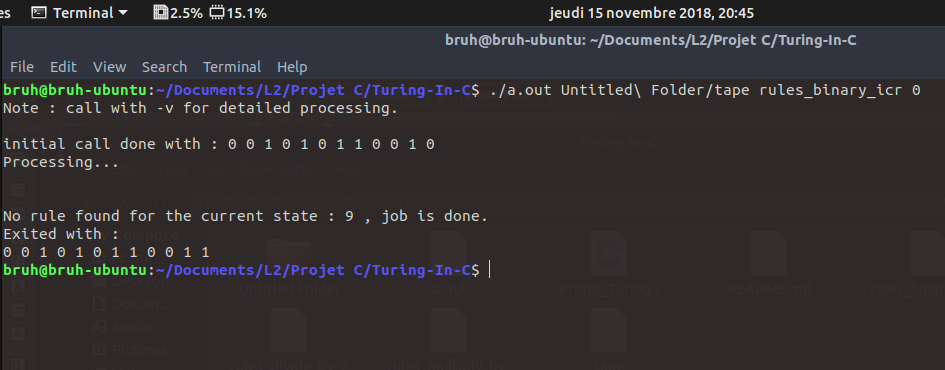
\includegraphics[scale=2.0]{screen1.png}
\\ \\
\subsection{Avec verbose}
Et un autre, toujours une incrémentation binaire, avec verbose. :

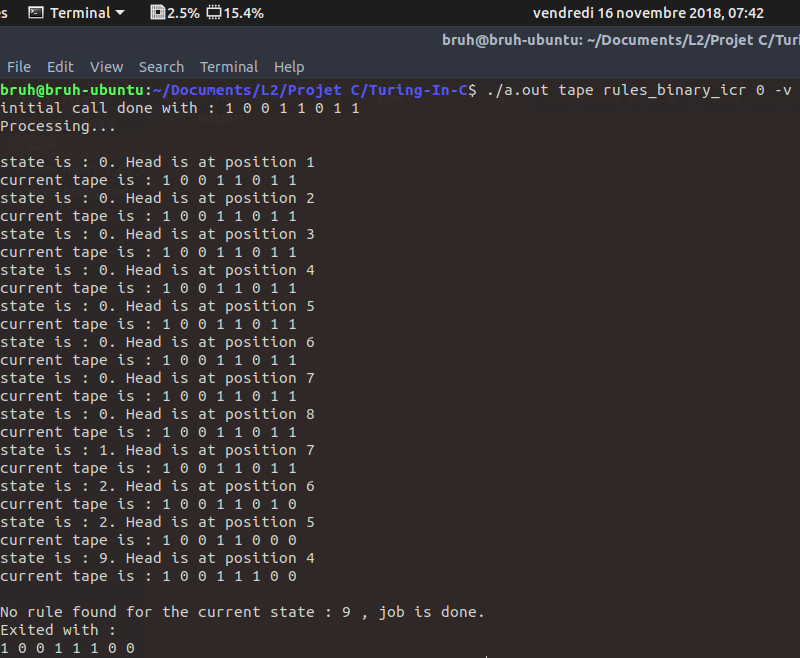
\includegraphics[scale=1.9]{screen2.png}

\section{Améliorations possibles}
On pourrait ajouter : 
\begin{itemize}
\item Une interface graphique
\item Un système permettant d'utiliser n'importe quel caractère plutot que des chiffres binaires
\item Une manière plus propre de gèrer les retenues...
\end{itemize}


\end{document}
